\documentclass{beamer}
\usetheme{madrid}
\title{lab 4}
\subtitle{jj}
%!!!!subtitle
\author{20513322}
\date{today}
\begin{document}
\begin{frame}
\maketitle
\end{frame}
\frametitle{outline}
\begin{frame}
\tableofcontents
\end{frame}
\section{introduction}
\begin{frame}
\frametitle{First order derivative}
\begin{block}{Station}
$x_0$is a stationary point
\end{block}
\end{frame}
\begin{frame}
\frametitle{Second order derivative}
\begin{block}{Second}
\begin{itemize}
\item x
\item y
\end{itemize}
\end{block}
\end{frame}
\section{Example}
\begin{frame}
Find local \textbf{maximum/minimum},\underline{Solution}:
\begin{equation}
f(x)=3x^4-20x^3+36x^2-18
\end{equation}
\end{frame}
\section{Application}
\begin{frame}
\begin{figure}[h]
\centering
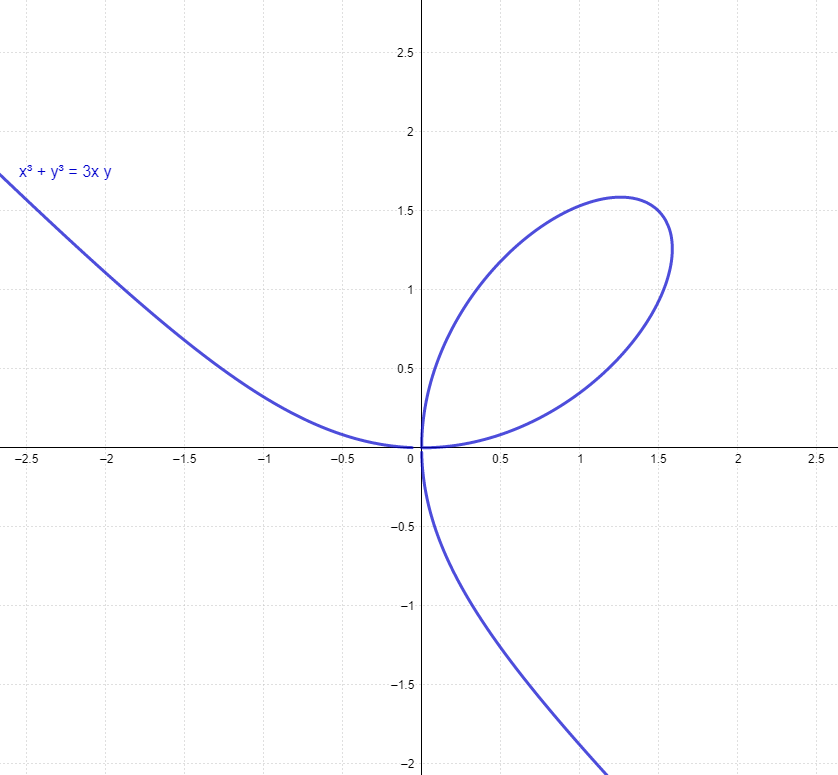
\includegraphics[scale=0.1]{eqnfig}
\caption{a}
\label{2}
%!!!!!label在caption后
\end{figure}
\end{frame}
\begin{frame}
	\begin{table}[h]
		\centering
		\begin{tabular}{|c|c|}
		$(x_0,f(x_0))$&h\\
		\end{tabular}
		\caption{h}
		\label{2}
	\end{table}
\end{frame}

\begin{frame}
\begin{columns}
%!!!没有数量
\column{0.5\textwidth}
%!!!没有begin
		\begin{eqnarray}
		x_{n-1}&=&x_n-\frac{f(x)}{f'(x)}\\
		&=&\cdots\nonumber
		\end{eqnarray}
\column{0.6\textwidth}
		\begin{tabular}{|c|c|}
		\hline
		n&$x_n$\\
		xss&r\\
		\hline
		\end{tabular}
\end{columns}
\end{frame}
%下标要在数学环境,column的用法
\begin{frame}
\frametitle{j}
\begin{columns}
\column{0.3\textwidth}
\begin{equation}
x^2=1
\end{equation}
\column{0.3\textwidth}
\begin{table}[h]
\centering
\begin{tabular}{|c|}
\hline
cc\\
\hline
\end{tabular}
\caption{h}
\end{table}
\end{columns}
\vfill
\end{frame}
\begin{frame}[fragile]
%!!!!!fragile放在这
\begin{verbatim}
\begin{eqnarray}
x_{n+1}&=& x_n-\frac{f(x_n)}{f’(x_n)}\\[1ex]
&=& \cdots \nonumber\\[1ex]
&=& \frac{9x_n^4-40x_n^3+36x_n^2+15}{12x_n^3-60x_n^2+72x_n}
\end{eqnarray}
\end{verbatim}
\end{frame}
\begin{frame}[fragile]\frametitle{Remark} % Frame 9
The iteration formula in \hyperlink{frame:fig}{\beamerbutton{previous frame}} is typeset by the following command lines:\\
\begin{verbatim}
\begin{eqnarray}
x_{n+1}&=& x_n-\frac{f(x_n)}{f'(x_n)}\\[1ex]
&=& \cdots \nonumber\\[1ex]
&=& \frac{9x_n^4-40x_n^3+36x_n^2+15}{12x_n^3-60x_n^2+72x_n}
\end{eqnarray}
\end{verbatim}
\end{frame}
































\end{document}